\section{Distributed Implementations}
\label{implementation}

To handle extremely large graphs and large amount of queries, we implement decentralized search on a distributed general graph processing platform, Powergraph~\cite{180251}. As decentralized search has low online search space complexity and have very low data dependency upon each other, it is well suited to run multiple searches in a parallel way. 

\begin{figure*}[ht]
    \centering
    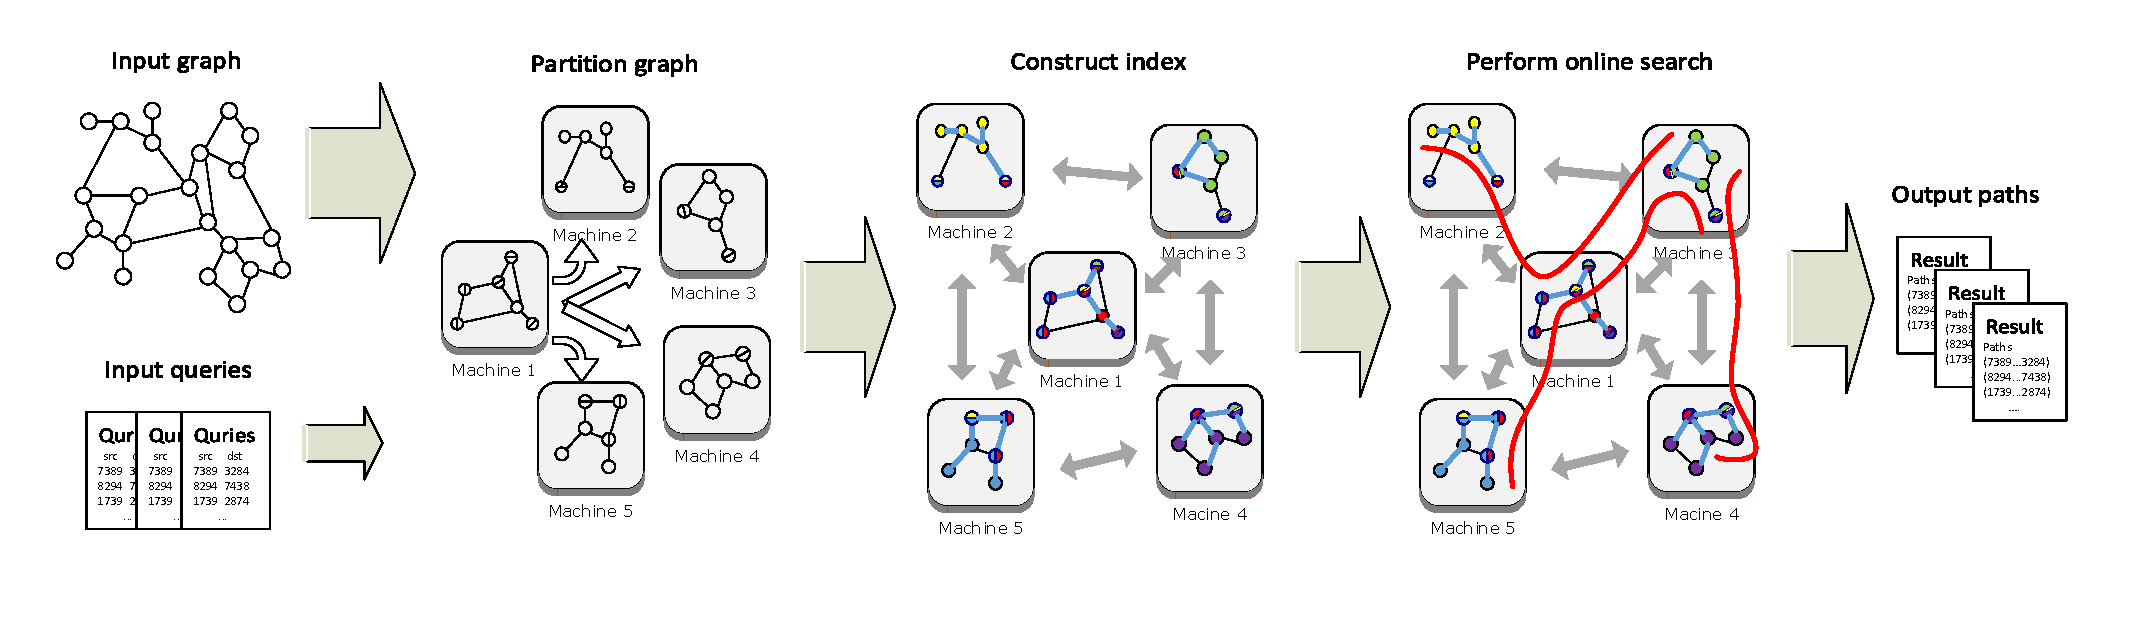
\includegraphics[width=\linewidth]{./figures/new_illustrate/system.pdf}
    \caption{A overview of distributed shortest path query processing system}
    \label{fig:system}
\end{figure*}

An overview of our shortest path query processing system is shown in Fig.~\ref{fig:system}. The system first partition the graph with Powergraph onto multiple machines. Then several BFSs are performed to construct the index. After the index has been built, multiple shortest path queries can run in parallel with decentralized search. Large volumes of queries can submit repeatedly, for which responses will be generated.

\subsection{Decentralized search vertex-program}

Decentralized search can be easily implemented as vertex-programs in Gather-Apply-Scatter model used by Powergraph. Index is stored distributively as vertex data. Each query instance contains the approximated path and label of target vertex, as it is not accessible on each machine locally. Each step of decentralized search is split into gather, apply and scatter phase. In Gather phase, LCA distance to target vertex $d_{LCA}$ is collected from each neighbor and accumulated by finding the neighbor with the smallest LCA distance to target. The accumulated result is returned as a next step candidate. In apply phase, the candidate is appended to the approximated path $p_{appr.}$ and the termination condition is checked. If it is met, the result path will be recorded and the query will be terminated. Otherwise, program will proceed to scatter phase to start a new vertex-program on the candidate vertex and pass on the query instance to them. Algorithm~\ref{alg:vc_dec} shows the detailed algorithm.

\begin{algorithm}
    \caption{Decentralized search vertex program on $u$}
		\label{alg:vc_dec}
    \begin{algorithmic}
        \Function{gather}{$L(v), L(t)$} 
						\Comment {on neighbor vertex $v$}
						\State \Return $d_{LCA}(v, t)$, $v$
				\EndFunction

        \Function{sum}{$d_{LCA}(v_1,t)$, $v_1$, $d_{LCA}(v_2,t)$, $v_2$}
						\If {$d_{LCA}(v_1,t) \le d_{LCA}(v_2,t)$}
								\State \Return $d_{LCA}(v_1,t), v_1$
						\Else
								\State \Return $d_{LCA}(v_2,t), v_2$
						\EndIf
				\EndFunction

        \Function{apply}{$L(t)$, $\tilde{p}(s,t)$, $d_{LCA}(v,t)$}
						\If {$v \in L(t)$}
								\State $p_{remain} \gets$ path from $v$ to $t$ in $L(t)$
								\State append $p_{remain}$ to $\tilde{p}(s,t)$
								\State store $\tilde{p}(s,t)$
								\State $term$ = true
						\Else
								\State append $v$ to $\tilde{p}(s,t)$
								\State $term$ = false
						\EndIf
				\EndFunction

        \Function{scatter}{$L(t)$, $\tilde{p}(s,t)$, $term$}
						\If {$\neg term$}
								\State Activate($v$, $L(t)$, $\tilde{p}(s,t)$)
						\EndIf
        \EndFunction
    \end{algorithmic}
\end{algorithm}

The communication for the decentralized search happen during gather and scatter phase. In gather phase, the label of target vertex need to be passed to multiple machines, and the size is $O(k{\sigma}_{max})$. And each gather function return a $d_{LCA}$ along side of its id. So for each query, only $O(k{\sigma}_{max})$ size of data is transferred. In scatter phase, communication happens when a vertex is chosen as the next step candidate and need to be activated, the whole search instance, including approximated path and label of target vertex need be transmitted to the new vertex program. For each query, $O(k{\sigma}_{max})$ size of data may be transferred. The search will take as much as $2{\sigma}_{max}$ steps. So the overall communication overhead for each query is $O(k{{\sigma}_{max}}^2)$. 

During decentralized search, only the approximated path $\tilde{p}$ is updated at each step. Therefore, there is only $RAR$ type of data dependency among multiple decentralized searches on the underlying graph. Depends on implementations, there may be output dependency, i.e. $WAW$, when output $\tilde{p}$ to the same container on each machine.

The low memory and communication cost, along side with $RAR$ only data dependency during the search makes a large number of decentralized search very suitable to run in parallel. To modify the vertex program for parallel processing, each vertex program maintain a list of search instance. During gather phase, label of target vertex for each query is transmitted to other machines, and $d_{LCA}$ is calculated for each query. Each query is updated during apply phase. In scatter phase, each query is examined for whether activating a certain vertex or not.

\subsection{Distributed tie breaking strategy}
According to tie breaking strategy, multiple neighbors may be returned as candidates at gather phase. In this case, the search instance copies itself into multiple search instances, append each candidate to each search instance at apply phase and activate them at scatter phase. The problem is, as search instances created at apply phase become independent when the search proceeding to next step, during the future steps, even one search instance find a shorter path than others, it can hardly terminate other searches as such synchronizations is too costly in distributed settings. With this limitation, a search may end up with excessive number of child search instances. To overcome this problem, in our implementation, only one candidate will be labeled as a "`main"' candidate at each step. For candidates that are not the "`main"' candidate, an extra termination condition is applied. In the next step, if the search cannot find a shorter path than expected, i.e. $|p_{appr.}| + d_LCA$, the search will stop, and no result will be recorded. This can control the search space effectively without compromise much accuracy.

\subsection{Prune LCA computation}
A major part of computation load of decentralized search is from large number of LCA computations. It is possible to prune number of LCA computation required at each step for decentralized search to reduce the overall computation load. Suppose the search is visiting vertex $u$, which means the $d_{LCA}(u, t)$ has already been calculated in previous step. If a neighbor $v$ is a child of $u$ on the indexed shortest path tree $SPT_l$, then the LCA computation for $v$ and $t$ on $SPT_l$ does not need to be performed as it is clearly that $d_{LCA_l}(v, t) > d_{LCA_l}(u, t)$. In practice, this principle can prune almost half of the total number of LCA computations of a single search on average.
